\section{Apparatus}
The brain speed-reader is an apparatus, which displays words on a screen at variable $r(t)$, which in turn is read by the user. The reading task triggers a change of brain activity, which can be recorded and analyzed through electroencephalograms (EEG). As our apparatus is conceived for use in a naturalistic environment, we have used, {\it Neurosky Mindwave}, the cheapest consumer-grade EEG headset available for less than \$100 on the market. As shown on Figure \ref{fig:apparatus} and explained step-by-step below, the EEG signal is processed online, in order to adapt the rate of words displayed as function of cognitive activity: if the rate $r$ is too large (resp. too low) at time $t$, then reading triggers more  (resp. less) cognitive activity, which in turn allows reducing (resp. increasing) $r$ at $t+1$. In this section, we explain step-by-step the design of the apparatus in details.

\begin{figure}[!t]
\centering
\includegraphics[width=0.9\columnwidth]{../figures/apparatus.eps}
\caption{Brain speed-reader apparatus: {\bf (a)} Words are displayed and read one after the other at a given rate. {\bf (b)} the EEG signal is recorded through a consumer grade device (here the {\it Neurosky Mindwave}). {\bf (c)} The EEG signal is turned every 0.5 seconds into a power spectrum through a Fourier transform, {\bf (d)} the characteristics of the power spectrum are compressed into a single value characteristic entropy $s$ value. {\bf (e)} A new rate of word display is updated by taking into its current value and $s$. {\bf (f)} The rate of word display is updated accordingly.}
\label{fig:apparatus}
\end{figure}

\subsection{Rate of Word Display}
The principle of {\it Rapid Serial Visual Presentation} (RVSP) applied to text, is precisely to display the words of a text at a controlled rate. However, in most RVSP implementations for text, the rate of word display pre-determined and remains constant. In our implementation, the user first calibrates the brain speed-reader by tuning a comfortable baseline word display rate $r_{baseline} = r(t = 0)$. The operation takes only a few seconds. This is a usual way to proceed when using usual text RVSP applications.

\subsection{Brain Activity as Captured by EEG signal}
Unlike traditional text RVSP, we wish to let the user adapt the rate of word display in real-time, through brain activity as captured by EEG signal, to control for a text becoming suddenly becoming more difficult, or just because the mindset of the user has changed, like sudden focus on an important part of the text (lower rate desired) or, on the contrary, loss of attention (higher rate of word displayed desired).

Because we want our apparatus be usable outside the lab, we have chosen the cheapest consumer-grade EEG scanner, available on the market for less than \$100.

\subsection{EEG Signal Processing}
One way to process the EEG signal, consists in analyzing its spectral properties over a determined period. Here, we take a time window of 0.25 second, which allows us to analyze the frequency domain $0-128Hz$, since the sampling rate of the Neurosky Mindwave is 512 measures per second (i.e., 512 Hz). Hence, every 0.25 second, we compute the power spectrum given by, 

 \begin{equation}
\label{eq:pspectrum}
\mathbf{[pspectrum~here]}
\end{equation}
 
and which is expected to approximately follow a power law, i.e., the probability to find a frequency $x$ is given by the probability density function $pdf(x)  = 1/x^{\mu+1}$. The power spectrum varies as a function of the mental tasks occurring, and potential external perturbations, such as voice, imperceptible and perceptible muscle movements, eye-movement, blinking.


\begin{figure}[!t]
\centering
\includegraphics[width=1.1\columnwidth]{../figures/compareArtifacts.eps}
\caption{Comparison of probability density functions (pdf, equiv. normalized power spectrum) for four typical tasks performed by one of the authors: (i) watching a screen, (ii) resting state, (iii) reading a text silently, (iv) making multiplications of 9 in silent (from 1x9 up to 15x9). For comparison, the standardized frequency ranges are also reported in colored areas. The pdfs are averaged over the length of the task with one power spectrum generated every second. For each task, the entropy values $s$ are reported, and we observe that $s$ is larger for more cognition intensive tasks. The behavior of $s$ can directly be rationalized by visual inspections  of the pdfs: One shall see the entropy as a measure of the $log(density)$ all over the pdf: for example, the reading task (red pdf) has the highest density on nearly all the frequency range. The multiplication task also exhibits high density all over the range, plus a large bump in the  (low + high) alpha frequency range and small bump in the high beta frequency range. These bumps explain why the multiplication task gets a larger entropy. Note that the resting state task exhibit the same bumps, but has lower log(density) in the theta and low alpha frequency ranges. Watching a screen has clearly the lowest log(density) all over the range. Usually, researchers only consider some frequency ranges, which are known to best discriminate between states of mind. Typically alpha and beta are most considered, and higher frequencies are not considered because they have low densities and are therefore polluted with noise, as it can clearly seen for frequencies higher that 60 Hz. Here, we contend that considering the whole pdf in logarithmic scale provides a more comprehensive view when comparing mind states, as shown on this figure, than slicing the pdf and only considering a few ranges. We can then apply standard tools, such as the entropy, for analyzing the probability density functions.}
\label{fig:pspectrum}
\end{figure}


Then, entropy.

\begin{equation}
\label{eq:tsallis}
S_q(X) = \frac{1}{q-1} \left( 1 - \sum_{i=1}^n (p_i)^q \right).
\end{equation}

\begin{equation}
\label{eq:shannon}
S_1(X) = - \sum_{i=1}^n p_i\cdot log_{2}(p_i), ~~for~~q=1.
\end{equation}

\subsubsection{Why Entropy ?}

higher frequencies are usually associated to higher cognitive brain activation. Higher activation  translated into larger entropy $S$.


We wanted a lightweight mobile apparatus, which does not require complicated machine learning or any communication with a cloud service, or would not drain a battery. We purposely decided for a cheap update method {\bf [continue this point in discussion because it helps introduce future work]}

\begin{figure}[!t]
\centering
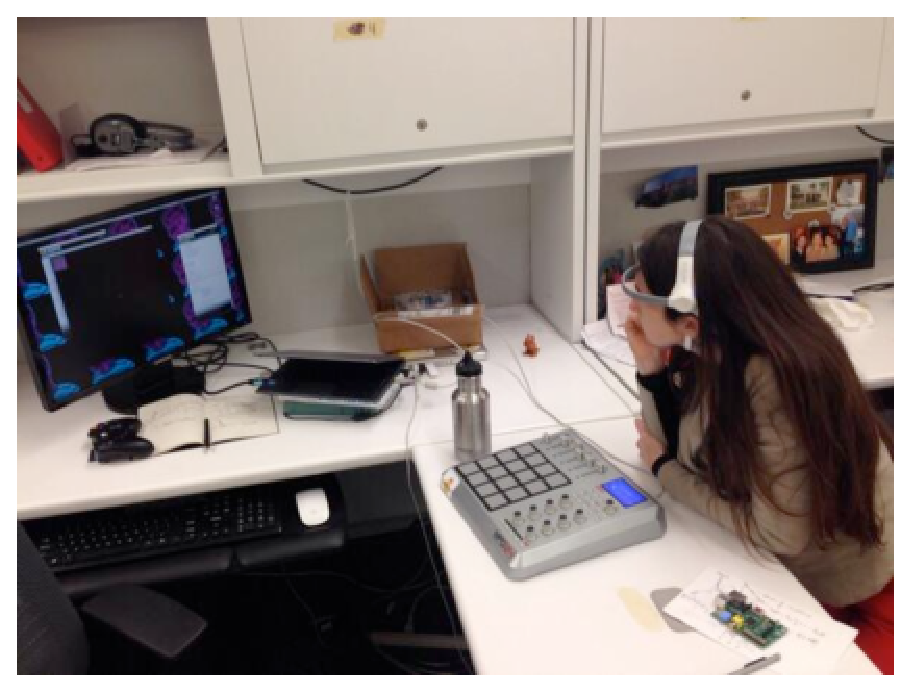
\includegraphics[width=0.9\columnwidth]{../figures/ariel.eps}
\caption{Ariel Garten (Interaxon / Muse CEO) playing with the brain speed reader.}
\label{fig:ariel}
\end{figure}

One could argue that we could have taken the {\it meditation} and {\it attention} metrics provided by Neurosky (and computed directly in the headset). However, these metrics are proprietary and their formula kept secret (we suspect nevertheless that they take $\alpha$ and $\beta$ waves  as an input). Furthermore, extensive testing did not allow us find any consistency with what we would quality meditation or attention. As a result, we preferred to stick to the principles of reproducible science.

\subsection{Negative Feedback Loop}

Explain: higher cog. activity  $\rightarrow$  higher entropy $\rightarrow$  lower word display rate $\rightarrow$ lower cog. activity. {\bf [probably not worth a section]}


\subsection{Word Display Rate Update}

\begin{equation}
\label{eq:Snormalized}
S_{norm}(t) = \frac{S(t) - \langle S \rangle}{\sigma_{S}}, 
\end{equation}
with $\langle S \rangle$ and $\sigma_{S}$ the average and standard deviation of the entropy $S$ calculated over the last 20 points (i.e., the last 5 seconds?). The normalization ensures that $S_{norm}$ is always centered around $0$. The rate $R(t+1)$ of word display is then updated as follows,

\begin{equation}
R(t+\Delta t) = R(t) \left[1 - \alpha \cdot S_{norm}(t)\right],
\label{eq:RateChange}
\end{equation}

where $\Delta t = 0.25$ seconds and $\alpha = 0.20$. In other words, the normalized entropy influences for 20\% the rate change $\Delta R =  \left[ R(t+\Delta t) - R(t) \right] / R(t) = - \alpha \cdot S_{norm}(t)$. Increasing $\alpha$ increases the influence of $S_{norm}$, and the negative sign ensures control of $R$ with a mean reverting process. Note however, that since $S_{norm}$ is calculated from a moving average on a rather short time window, $R$ exhibits excursions (c.f. Figure \ref{fig:trajectory}).

\begin{figure}[!t]
\centering
%\includegraphics[width=0.9\columnwidth]{../figures/apparatus.eps}
\caption{typical evolution of rate $R$.}
\label{fig:trajectory}
\end{figure}
